The first model is an initial approach using a VGG inspired architecture.
\begin{center}
    \begin{verbatim}
        Model: "sequential_4"
_________________________________________________________________
Layer (type)                 Output Shape              Param #   
=================================================================
conv2d_26 (Conv2D)           (None, 32, 32, 32)        896       
_________________________________________________________________
conv2d_27 (Conv2D)           (None, 32, 32, 32)        9248      
_________________________________________________________________
max_pooling2d_13 (MaxPooling (None, 16, 16, 32)        0         
_________________________________________________________________
conv2d_28 (Conv2D)           (None, 16, 16, 64)        18496     
_________________________________________________________________
conv2d_29 (Conv2D)           (None, 16, 16, 64)        36928     
_________________________________________________________________
max_pooling2d_14 (MaxPooling (None, 8, 8, 64)          0         
_________________________________________________________________
conv2d_30 (Conv2D)           (None, 8, 8, 128)         73856     
_________________________________________________________________
conv2d_31 (Conv2D)           (None, 8, 8, 128)         147584    
_________________________________________________________________
max_pooling2d_15 (MaxPooling (None, 4, 4, 128)         0         
_________________________________________________________________
flatten_4 (Flatten)          (None, 2048)              0         
_________________________________________________________________
dense_8 (Dense)              (None, 128)               262272    
_________________________________________________________________
dense_9 (Dense)              (None, 10)                1290      
=================================================================
Total params: 550,570
Trainable params: 550,570
Non-trainable params: 0
_________________________________________________________________
    \end{verbatim}
\end{center}
This is a VGG-style network with 3 blocks compromised of 2 convolution layers and a pooling layer, followed by a dense fully connected layer for classification.
The ReLU\footnote{\href{https://machinelearningmastery.com/rectified-linear-activation-function-for-deep-learning-neural-networks/}{https://machinelearningmastery.com/rectified-linear-activation-function-for-deep-learning-neural-networks/}} activation function is used at each layer, and the loss function of the network is Cross Entropy\footnote{\href{https://www.tensorflow.org/api\_docs/python/tf/keras/losses/CategoricalCrossentropy}{https://www.tensorflow.org/api\_docs/python/tf/keras/losses/CategoricalCrossentropy}}
The network is optimized using the Adam algorithm\footnote{\href{https://keras.io/api/optimizers/adam/}{https://keras.io/api/optimizers/adam/}}.
This model gave an accuracy of about 83\% after 50 epochs, but the learning curve indicates overfitting happening early on.
\begin{center}
    \captionsetup{type=figure}
    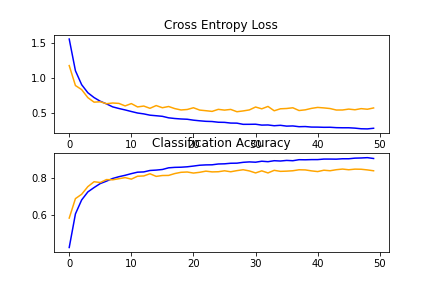
\includegraphics[width=250px]{sections/exp-2/images/initial-plot.png}
    \captionof{figure}{Experiment 2 - Model 1 - Cross Entropy Loss \& Classification Accuracy}
\end{center}
The problem of overfitting will be addressed the second model, by introducing dropout in the network, we will also attempt to increase prediction accuracy by introducing batch normalization and another dense classification layer.
